\makeatletter
\def\input@path{{../}}
\makeatother
\documentclass[../master_thesis.tex]{subfiles}
\begin{document}
\chapter{Implementation}\label{chap:implementation}
\section{Fosso-Tande \& Harrison's \ac{GPE}}
Fosso-Tande and Harrison described in \cite{FossoTande:2013ka} a \ac{GPE} that
included a dielectric function which was analytical through the cavity boundary.
This model was explained with more detail in chapter \ref{Solvent_effect} and
it will not be explained again, here we will show how it was implemented on
\mrchem.
\subsection{Cavity Function}
The first step was to create a cavity function as in \cite{FossoTande:2013ka}.
This was done by creating a cavity object that stored the coordinates of nuclei
$\rvec_I$ and their characteristic radii $R_I$. When a point $\rvec$ is evaluated
in the Cavity function it will return $0$ if it is outside the cavity and $1$ if
it is inside the Interlocking spheres cavity defined by the nuclei coordinates
and their radii. Additionally we wanted to be able to change the width of the
boundary $\sigma$. The structure of the cavity object is as in Algorithm \ref{alg:Cavity}

\begin{algorithm}
  \caption{Cavity object}\label{alg:Cavity}
  \begin{algorithmic}
    \STATE \underline{\textbf{Initialize $C(\rvec)$}}
    \STATE \textbf{Input :} Coordinates, Radii, Width
    \STATE $\sigma = $ Width
    \STATE $C_{tot}(\rvec) = 1$
    \FOR{ All Coordinates and Radii $I$}
     \STATE $\rvec_I = $ Coordinate$_I$
     \STATE $R_I = $ Radius$_I$
    \ENDFOR
    \STATE
    \STATE \underline{\textbf{Evaluate $C(\rvec)$}}
    \STATE \textbf{Input: } $\rvec$
    \FOR{All $I$}
      \STATE $s_I(\rvec) = \abs{\rvec - \rvec_I} - R_I$
      \STATE $\Theta_I(\rvec) = \frac{1}{2}\left(1 + \erf\left(\frac{s_I(\rvec)}{\sigma}\right)\right)$
      \STATE $ C_I(\rvec) = 1 -\Theta_I(\rvec) $
      \STATE $ C_{tot}(\rvec) = C_{tot}(\rvec) \cdot (1 - C_{I}(\rvec))$
    \ENDFOR
    \RETURN $ 1 - C_{tot}(\rvec)$
  \end{algorithmic}
\end{algorithm}
This Object was implemented as a derived class of \verb!RepresentableFunction!,
a C++ class in \mrchem.
\subsection{Dielectric Function}
In Equations \ref{eq:dielfunclin} and \ref{eq:dielfuncexp} we defined both a
linear $\epslin$ and exponential $\epsexp$ dielectric function. These were implemented as presented
in those two equations, with no changes to them, except for minor syntax related
adjustments. Their $\log$ derivatives had to be implemented separately,
this was done in order to have better convergence \cite{FossoTande:2013ka}. The
$\log$ derivative of the exponential dielectric function is represented as the
derivative of the Cavity multiplied by a constant. The cavity of Water as implemented
above can be seen in Figure \ref{fig:watcav} as a slice through the $xz$ plane.

\begin{figure}[ht]
  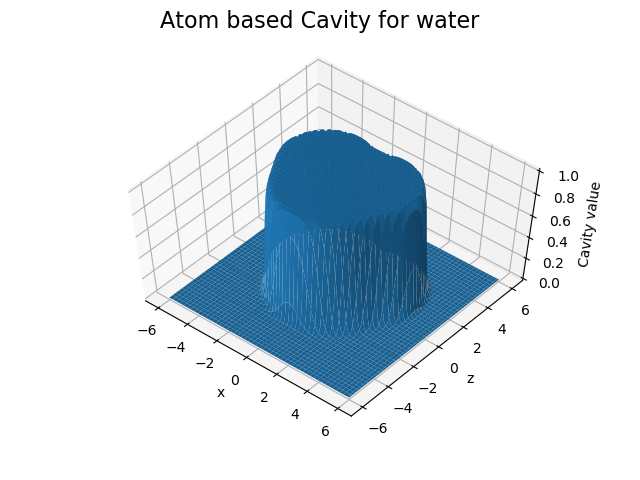
\includegraphics[width=\linewidth]{img/Figure_1-1.png}
  \caption{Interlocking spheres cavity slice for water}
  \label{fig:watcav}
\end{figure}

\subsection{Effective volume charge distribution}
When Running a \ac{SCF} calculation one calculates with electron densities in order
to solve an electron \SE as is consistent with the \ac{BO} approximation
\cite{Cramer:2004, Konishi:2009}, whereas Fosso-Tande and Harrison's \ac{GPE}
needs the total molecular density $\rho_{tot}$. This is computed as a sum of the electron
density $\rho_{el}$ and a computed nuclear density $\rho_{nuc}$ based on the '
geometry and charge of the nuclei
\begin{equation}
  \rho_{tot} = \rho_{el} + \rho_{nuc}
\end{equation}.
The following algorithm \ref{alg:rhonuc} shows how we calculate the nuclear
density $\rho_{nuc}$ for the total density by use of Gaussian functions centered at
each nucleus.
\begin{algorithm}
  \caption{Nuclear charge density}\label{alg:rhonuc}
  \begin{algorithmic}
    \STATE \textbf{Input :} Nuclear coordinates, Charges
    \STATE $\alpha = 1000$
    \STATE $\beta = (\frac{\alpha}{\pi})^{\frac{3}{2}} \cdot \text{Charge}_I$
    \STATE $\rvec_I(\rvec) =$ Nuclear coordinate$_I$
    \STATE $\rho_{nuc} = 0$
    \FOR{All coordinates and charges $I$}
    \STATE $\rho_{nuc}^{(I)}(\rvec) = \beta e^{-\alpha\cdot\lVert\rvec -\rvec_I\rVert^2}$
    \STATE $\rho_{nuc(\rvec)} = \rho_{nuc(\rvec)} + \rho_{nuc}^{(I)}(\rvec)$
    \ENDFOR
    \RETURN $\rho_{nuc}(\rvec)$
  \end{algorithmic}
\end{algorithm}

Where $\alpha$ represents the width of the Gaussian function, $\beta$ is the normalization
constant multiplied with the charge, $\rvec_I$ is the position of the nucleus and
$\rho_{nuc}^{(I)}$ is the Gaussian representing the a point charge at the nucleus.
The algorithm \ref{alg:rhonuc} describes the set of nuclei as a sum of different point charges
represented as Gaussian functions.

We then go on to create the effective volume charge distribution by the following equation.
\begin{align}
    \begin{split}
      \rho_{eff} = \frac{1 - \epsilon}{\epsilon}\rho_{tot}\\
    \end{split}
\end{align}
This differs from Fosso-Tande's effective charge distribution in that we incorporate
the subtraction of $U_{vac}$ to it from the start \cite{FossoTande:2013ka}. This
way we will be solving directly for the reaction field potential $U_r$.
The alternative is to instead compute the total potential $U$ and then subtract
the gas phase potential to get the Reaction potential as in \cite{FossoTande:2013ka}.

\subsection{Surface Charge distribution}
Given the total interaction potential of $U$ of a solvation system with
dielectric function $\epsilon$ defined with cavity $C$, we compute the surface charge distribution
$\gamma_s$ as shown in algorithm \ref{alg:gamma}.
\begin{algorithm}
  \caption{Surface charge distribution}\label{alg:gamma}
  \begin{algorithmic}
    \STATE $\gamma_s[U, epsilon[C]]$:
    \STATE \textbf{Input :} $U$ potential, $\epsilon[C]$ dielectric function
    \IF{$\epsilon$ is exponential}
      \STATE $k = \frac{1}{4\pi}\log\frac{\epso}{\epsinf}$
      \RETURN $k \nabla C \cdot \nabla U$
    \ELSIF{$\epsilon$ is linear}
      \STATE $k = \frac{1}{4\pi}\epso-\epsinf$
      \RETURN $\frac{k}{\epsilon} \nabla C \cdot \nabla U$
    \ENDIF
  \end{algorithmic}
\end{algorithm}

Here we use the definition of the log derivative for both $\epslin$ and $\epsexp$
from equations \ref{eq:logderepsexp} and \ref{eq:logderepslin}. This is the same
as just writing $$\gamma_s = \frac{1}{4\pi}\frac{\nabla\epsilon\nabla U}{\epsilon}$$,
which is the same equation as in \ref{eq:effrhogamma}.

\subsection{The iterative \ac{SCRF} method}
In this method we Compute the Reaction field of the solvation system by iteration.
Here we follow the equation for the Reaction field potential in section \ref{solmw}.
In that section we see that, in order to compute the reaction potential, we need
to compute the surface charge distribution of the reaction potential. This
paradox is resolved by an iterative process. In this section I will explain how
this process works.

The first potential that is calculated will be a gas phase potential $U_{vac}$ this
potential is found by applying the Poisson operator $\hat{\mathscr{P}}$ defined
in Equation \ref{eq:Poissonopmw} on only the total charge density $\rho_{tot}$.
This is then used to make the zeroth Surface charge distribution $\gamma_s^{(0)}$.
This zeroth gamma is then added to the effective volume charge distribution $\rho_{eff}$
and the Poisson operator is applied to the sum in order to get the reaction potential.
This reaction potential is then used next iteration if the \ac{SCRF} to compute
the first surface charge distribution, which is then used to compute the next
and so on. This is done until the norm of the difference between the previous
reaction potential and the new one is less than a user defined precision. This is shown in
Algorithm \ref{alg:Reactionfield}.
\begin{algorithm}
  \caption{\ac{SCRF} iterative method}\label{alg:Reactionfield}
  \begin{algorithmic}
    \STATE \underline{\textbf{Zeroth iteration:}}
    \STATE $U_{vac} = \hat{\mathscr{P}}(\rho_{tot})$
    \STATE $\gamma_s^{(0)} = \gamma_s\big[U_{vac}, \epsilon\big]$
    \STATE $U_r^{(1)} = \hat{\mathscr{P}}(\rho_{eff} + \gamma_s^{(0)})$
    \STATE \underline{\textbf{n-th iteration:}}
    \STATE \textbf{Input :} precision
    \STATE error = 10
    \WHILE{error $\geqslant$ precision}
      \STATE $\gamma_s^{(n)} = \gamma_s\big[(U_{vac}+ U_r^{(n)}), \epsilon\big]$
      \STATE $U_r^{(n+1)} = \hat{\mathscr{P}} (\rho_{eff} + \gamma_s^{(n)})$
      \STATE error = $\lVert U_r^{(n+1)} - U_r^{(n)} \rVert$
      \STATE $U_r^{(n)} = U_r^{(n+1)}$
    \ENDWHILE
    \RETURN $U_r^{(n)}$
  \end{algorithmic}
\end{algorithm}
The \ac{SCRF} can then be implemented by itself or in-between every normal
\ac{SCF} cycle. The converged Reaction potential for water in a water solvent
can be seen in Figure \ref{fig:watpots}.

\begin{figure}[h!]
  \centering
  \begin{subfigure}[b]{0.49\linewidth}
    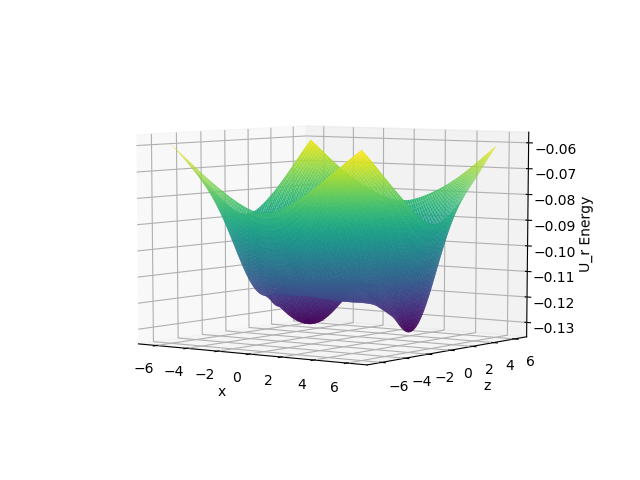
\includegraphics[width=\linewidth]{img/Urpot5.png}
  \end{subfigure}
  \begin{subfigure}[b]{0.49\linewidth}
    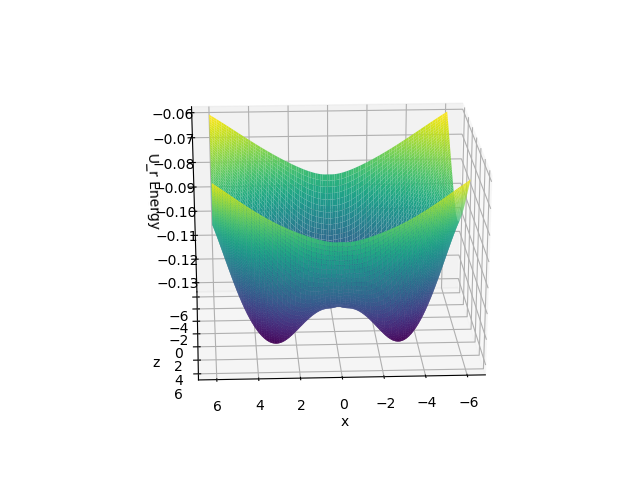
\includegraphics[width=\linewidth]{img/Urpot2.png}
  \end{subfigure}
  \begin{subfigure}[b]{0.49\linewidth}
    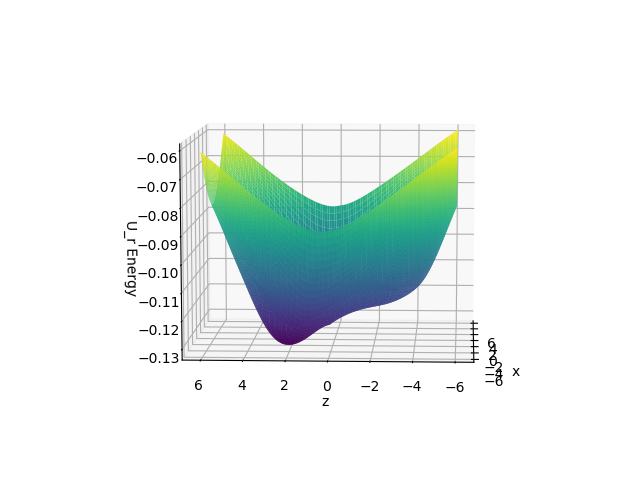
\includegraphics[width=\linewidth]{img/Urpot3.png}
  \end{subfigure}
  \begin{subfigure}[b]{0.49\linewidth}
    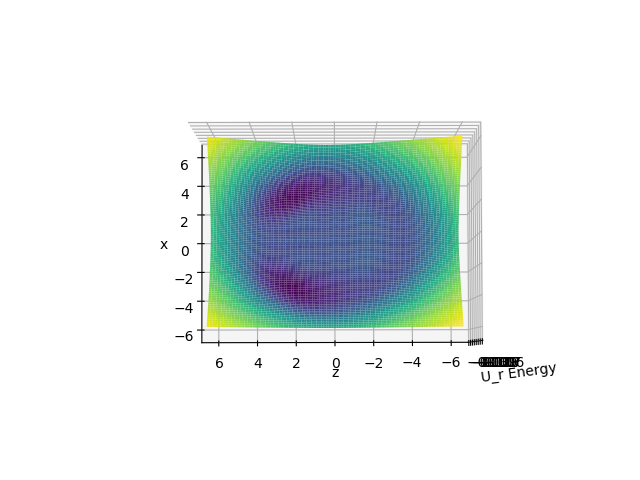
\includegraphics[width=\linewidth]{img/Urpot4.png}
  \end{subfigure}
  \begin{subfigure}[b]{\linewidth}
    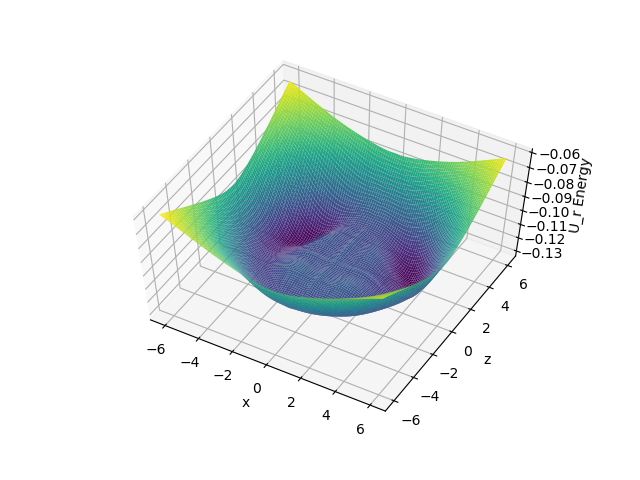
\includegraphics[width=\linewidth]{img/Urpot1.png}
  \end{subfigure}
  \caption{Reaction potential plotted for the xz plane}
  \label{fig:watpots}
\end{figure}

\section{Variational implementation}
The variational implementation is very similar to the iterational one described.
All the steps outlined above are the same during the first \ac{SCF} cycle. Except
that in the end, we compute the next $\gamma_s^{(n)}$ with the converged $U_r$ before
moving on to the next \ac{SCF} cycle. This $\gamma_s^{(n)}$ is then used in the next cycle
to compute only one iteration of the \ac{SCRF} without checking the error against the
precision. After the one iteration we use the new $U_R$ to compute the $\gamma_s^{(n+1)}$
for the next iteration. If one is using a convergence accelerator one can make
use of the old surface charge distribution $\gamma_s^{(n)}$ and the new one just computed
$\gamma_s^{(n+1)}$ to accelerate the convergence of the Reaction field potential.
This is outlined in algorithm \ref{alg:Reactionfieldvar}.
\begin{algorithm}
  \caption{\ac{SCRF} variational method}\label{alg:Reactionfieldvar}
  \begin{algorithmic}
    \STATE \underline{\textbf{Zeroth step:}}
    \STATE Do The iterative \ac{SCRF} $\rightarrow U_r^{(converged)}$
    \STATE $\gamma_s^{(n+1)} = \gamma_s\big[(U_{vac}+ U_r^{(converged)}), \epsilon\big]$
    \STATE \underline{\textbf{n-th step:}}
    \FOR{Every \ac{SCF} cycle do:}
      \STATE $\gamma_s^{(n)} =\gamma_s^{(n+1)}$
      \STATE $U_r^{(n)} = \hat{\mathscr{P}} (\rho_{eff} + \gamma_s^{(n)})$
      \STATE $\gamma_s^{(n+1)} = \gamma_s\big[(U_{vac}+ U_r^{(n)}), \epsilon\big]$
      \STATE $U_r^{(n)} = U_r^{(n+1)}$
      \STATE $\gamma_s^{(n+1)} = \gamma_s\big[(U_{vac}+ U_r^{(converged)}), \epsilon\big]$
      \STATE Accelerator[$\gamma_s^{(n)}, \gamma_s^{(n+1)}] \rightarrow \gamma_s^{(n+1)\prime}$
      \STATE $\gamma_s^{(n+1)} =\gamma_s^{(n+1)\prime}$
    \ENDFOR
  \end{algorithmic}
\end{algorithm}
Where $\gamma_s^{(n+1)\prime}$ is an optimized $\gamma_s^{(n+1)}$ which is used
in the next iteration. The first Iterative \ac{SCRF} was done so that we would
start the Optimizing of the potential with an already good guess.
\section{Software used}
The problem was first implemented in Vampyr %cite and get the right font
which is a python %
Then it was implemented in C++ using \mrchem %cite and get the right font
Both implementations are identical, except for slight changes for
performance improvement, such as a KAIN accelerator, %cite and correct font
iterating through $U_r$ instead of $U_{tot}$ % more explanation on this in previous or this section
and keeping the potential from cycle to cycle
in the c++ version of the model.


\begin{acronym}
\acro{AUS}[\href{https://www.sigma2.no/content/advanced-user-support}{AUS}]{Numerical Methods in Quantum Chemistry}
\acro{BO}{Born-Oppenheimer}
\acro{CTCC}[\href{http://www.ctcc.no}{CTCC}]{Centre for Theoretical and Computational Chemistry}
\acro{DC}{Dielectric Continuum}
\acro{DFT}{Density Functional Theory}
\acro{EFP}{Effective Fragment Potential}
\acro{EU}{European Union}
\acro{HF}{Hartree-Fock}
\acro{Hylleraas}[\href{https://www.mn.uio.no/hylleraas/english/}{Hylleraas}]{Hylleraas
  Centre for Quantum Molecular Sciences}
\acro{HPC}{High Performance Computing}
\acro{KTH}{Royal Institute of Technology}
\acro{LDA}{Local Density Approximation}
\acro{MCD}{Magnetic Circular Dichroism}
\acro{MCSCF}{Multiconfiguration Self Consistent Field}
\acro{MM}{Molecular Mechanics}
\acro{MW}{Multiwavelet}
\acro{NFR}{Norwegian Research Council}
\acro{NMQC}[\href{http://www.ctcc.no/events/conferences/2015/numeric-conference/}{NMQC}]{Numerical Methods in Quantum Chemistry}
\acro{NOTUR}[\href{https://www.notur.no/}{NOTUR}]{Norwegian Metacenter for Computational Science}
\acro{PCM}{Polarizable Continuum Model}
\acro{PI}{Primcipal Investigator}
\acro{QC}{Quantum Chemistry}
\acro{QM}{Quantum Mechanics}
\acro{QM/MM}{Quantum Mechanics/Molecular Mechanics}
\acro{ROA}{Raman Optical Activity}
\acro{SC}{semiconductor}
\acro{SCF}{Self Consistent Field}
\acro{SHG}{Second Harmonic Genertation}
\acro{STSM}{Short-term scientific mission}
\acro{TPA}{Two-Photon Absorption}
\acro{WP}{Work Package}
\acro{CBS}{Complete Basis Set}
\acro{TCG}{Theoretical Chemistry Group}
\acro{vdW}{van der Waals}
\acro{SE}{Schrödinger Equation}
\acro{PES}{Potential Energy Surface}
\acro{LCAO}{Linear Combination of Atomic Orbitals}
\acro{MRA}{Multi-Resolution Analysis}
\acro{NS}{Nonstandard}
\end{acronym}

\biblio
\end{document}
